\documentclass[12pt]{article}
\usepackage[margin=1in]{geometry}
\usepackage{fancyhdr}
\usepackage{amsmath}
\usepackage{amssymb}
\usepackage{bbm}
\usepackage{float}
\usepackage{xspace}
\usepackage{color}
\usepackage{graphicx}
\usepackage{caption,subcaption}
\usepackage[ruled]{algorithm2e}
\usepackage[backend=biber,style=apa]{biblatex}
\usepackage[colorlinks=true,allcolors=black,linkcolor=blue,urlcolor=blue]{hyperref}


\pagestyle{fancy}
\fancyhf{}
\rhead{\footnotesize{STAT520B Project Report --- pg. \thepage}}
\renewcommand{\headrulewidth}{0pt}

\setlength\parindent{0pt}

\newcommand{\todo}{\textcolor{red}{TODO}}

\newcommand{\vsmc}{\textsc{VSMC}\xspace}
\newcommand{\uvsmc}{\textsc{uVSMC}\xspace}
\newcommand{\gsvsmc}{\textsc{GS-VSMC}\xspace}
\newcommand{\igrvsmc}{\textsc{IGR-VSMC}\xspace}
\newcommand{\smc}{\textsc{SMC}\xspace}
\newcommand{\mcmc}{\textsc{MCMC}\xspace}
\newcommand{\kl}{\textsc{KL}\xspace}
\newcommand{\elbo}{\textsc{ELBO}\xspace}
\newcommand{\categorical}{\textsc{Categorical}\xspace}
\newcommand{\grep}{g_{\mathrm{rep}}}
\newcommand{\gscore}{g_{\mathrm{score}}}
\newcommand{\gumbelsoftmax}{\textsc{Gumbel-Softmax}\xspace}
\newcommand{\gumbel}{\textsc{Gumbel}\xspace}
\newcommand{\gaussian}{\textsc{Gaussian}\xspace}
\newcommand{\igr}{\textsc{IGR}\xspace}
\newcommand{\iwae}{\textsc{IWAE}\xspace}
\newcommand{\ssm}{\textsc{SSM}\xspace}
\newcommand{\capm}{\textsc{Capm}\xspace}

\DeclareMathOperator{\surrogate}{\tilde{\mathcal{L}}}
\DeclareMathOperator*{\argmin}{arg\,min}

% References
\bibliography{refs.bib}
\setlength\bibitemsep{1.5\itemsep}


\title{\vspace{-1.5cm}\textbf{Fully Reparameterized \\ Variational Sequential Monte Carlo}}
\author{Kenny Chiu}
\date{}


\begin{document}

\maketitle
\thispagestyle{fancy}

\begin{abstract}
We review the main contributions and limitations of the original Variational Sequential Monte Carlo paper by \textcite{Naesseth:2018}. We also propose a modification to the Variational Sequential Monte Carlo algorithm where we replace the \categorical resampling step with a continuous, reparameterizable approximation in order to reduce the variance of the unbiased \elbo gradient estimator. Our empirical results suggest that using the \gumbelsoftmax approximation reduces the variance of the unbiased estimator and achieves a performance comparable to that of the biased gradient estimator. We also see potential with the Invertible Gaussian Reparameterization, but it has computational limitations that need to be first addressed.
\end{abstract}

\section{Introduction}

The paper by \textcite{Naesseth:2018} introduces Variational Sequential Monte Carlo (\vsmc) as a flexible variational family for approximating the posterior distribution of a sequence of random variables. In this project, we discuss the main contributions and limitations of the paper. We also review \vsmc and propose a fully reparameterized version of \vsmc aimed at addressing its problems of noisy gradient estimation. We evaluate our proposed extension through experiments similar to those in the original paper.
\\

This report is organized as follows: Section~\ref{sec:vsmc} reviews the paper and \vsmc; Section~\ref{sec:approx} describes our proposed modification to \vsmc; Section~\ref{sec:experiments} discusses the results of our experiments that evaluate our proposed modifications; and Section~\ref{sec:discussion} summarizes our main points and concludes with a discussion of what we have learned.


\section{Variational Sequential Monte Carlo}\label{sec:vsmc}

The main contributions of the paper by \textcite{Naesseth:2018} include the introduction of the \vsmc variational family, as well as the derivation of a tractable bound for optimizing \vsmc. Following \parencite{Naesseth:2018}, we provide an overview of these ideas in the context of a state space model (\ssm). Let $x_{1:T}$ and $y_{1:T}$ denote sequences of $T$ latent variables and $T$ observations, respectively, and assume that their joint distribution factorizes as
\[
p(x_{1:T},y_{1:T}) = p(x_1)\prod_{t=2}^Tp(x_t|x_{t-1})\prod_{t=1}^Tp(y_t|x_t) \;.
\]
The target distribution is then the posterior distribution $p(x_{1:T}|y_{1:T})$.

\subsection{Sequential Monte Carlo}

\vsmc is heavily based on Sequential Monte Carlo (\smc). \smc is a \mcmc method that approximates the posterior distribution of a sequence of random variables using a set of $N$ weighted particles. \smc constructs the set of particles through the following procedure:
\begin{enumerate}

\item
Initialize $N$ samples $x_1^{1:N}$ from some proposal distribution $q(x_1)$ and assign a weight $w_1^i=\frac{p(x_1^i)p(y_1^i|x_1^i)}{q(x_1^i)}$ to each sample $x_1^i$, $i=1,...,N$.

\item
For iterations $t=2,...,T$, do the following three steps:
\begin{enumerate}

\item
\textbf{Resample}: sample \textit{ancestor} variables $a_t^i\in\{1,...,N\}$, $i=1,...,N$, from a \categorical distribution with probabilities proportional to $w_{t-1}^{1:N}$.

\item
\textbf{Propose}: propose new states $x_t^i$, $i=1,...,N$, according to some proposal distribution $q(x_t^i|x_{t-1}^{a_t^i})$.

\item
\textbf{Reweight}: assign new weights $w_t^i=\frac{p(x_t^i|x_{t-1}^{a_t^i})p(y_t^i|x_t^i)}{q(x_t^i|x_{t-1}^{a_t^i})}$, $i=1,...,N$, to each new state $x_t^i$.

\end{enumerate}

\end{enumerate}

Let $x_{1:T}^i$, $i=1,...,N$ denote the sequence of states that gave rise to $x_T^i$, i.e.,
\[
x_{1:T}^i=\left(x_1^{\ldots},\ldots, x_{T-2}^{a_{T-1}^{a_{T-2}^{\ldots}}}, x_{T-1}^{a_T^i}, x_T^i\right) \;.
\]
The above procedure returns the set of particles $x_{1:T}^{1:N}$ along with weights $w_T^{1:N}$. \smc then approximates the posterior distribution with the discrete measure
\[
p(x_{1:T}|y_{1:T}) \approx q(x_{1:T}|y_{1:T}) \overset{\Delta}{=} \sum_{i=1}^N\frac{w_T^i}{\sum_{\ell=1}^Nw_T^\ell}\delta_{x_{1:T}^i}
\]
where $\delta_x$ is the Dirac measure at $x$. Notice that the approximation $q(x_{1:T}|y_{1:T})\rightarrow p(x_{1:T}|y_{1:T})$ as $N\rightarrow\infty$. Also note that while we cannot evaluate the density of the approximation, we can sample from it by sampling a particle $x_{1:T}^i$ with probability proportional to $w_T^i$.

\subsection{\vsmc Objective}

The key design choice of \smc is choosing the proposal distribution $q$. Instead of specifying a distribution, \vsmc postulates a parametric variational family $q_\lambda$ with variational parameters $\lambda$ for the proposal and learns the optimal proposal that minimizes
\[
\mathrm{KL}\left(q_\lambda(x_{1:T}|y_{1:T})\| p(x_{1:T}|y_{1:T})\right) \;.
\]
This objective and the corresponding evidence lower bound (\elbo) is intractable, however, due to the intractable posterior density of $q_\lambda$. \textcite{Naesseth:2018} derive a \textit{surrogate} \elbo given by
\[
\surrogate(\lambda) \overset{\Delta}{=} \mathbb{E}_{x_{1:T}^{1:N},a_{2:T}^{1:N}}\left[\log \hat{p}(y_{1:T})\right]
\]
where $\hat{p}(y_{1:T})$ is an unbiased estimator of $p(y_{1:T})$ and is given by
\[
\hat{p}(y_{1:T}) = \prod_{t=1}^T\frac{1}{N}\sum_{i=1}^Nw_t^i \;.
\]
The surrogate \elbo is a lower bound to the \elbo and can be optimized stochastically using samples obtained from running \smc. Assuming that the proposal $q_\lambda(x_t|x_{t-1})$ can be reparameterized in terms of some noise distribution $p(\varepsilon_t)$ independent of the parameters $\lambda$, the gradient of the surrogate \elbo can then be rewritten as
\begin{align*}
\nabla\surrogate(\lambda) &= \grep + \gscore \\
\grep &= \mathbb{E}_{\varepsilon_{1:T}^{1:N},a_{2:T}^{1:N}}\left[\nabla\log\hat{p}(y_{1:T})\right] \\
\gscore &= \mathbb{E}_{\varepsilon_{1:T}^{1:N}}\left[\log\hat{p}(y_{1:T})\nabla\log p_\lambda(a_{2:T}^{1:N}|\varepsilon_{1:T}^{1:N}) \right] \;.
\end{align*}
The $\gscore$ component is dependent on the \categorical distribution of the ancestors, which in turn is dependent on $\lambda$ through the weights $w_{1:T}^{1:N}$ and cannot be reparameterized. \textcite{Naesseth:2018} found that the stochastic estimator for $\gscore$ had a much larger variance compared to that of $\grep$, which impacts the convergence rate of the stochastic optimization. \textcite{Naesseth:2018} proposed several strategies to reduce the variance in practice, such as ignoring $\gscore$ (resulting in a biased gradient estimator), Rao-Blackwellization~\parencite{Robert:2021}, and using control variates. Overall, the noisy unbiased gradient estimator due to the ancestor variables being non-reparameterizable is the main limitation of \vsmc. We aim to address this issue with our proposed extension in Section~\ref{sec:approx}.

\subsection{Other Contributions and Limitations}

We conclude this section with a brief mention of the other contributions and limitations of the paper. \textcite{Naesseth:2018} also make a connection between \vsmc and Importance Weighted Autoencoders~\parencite{Burda:2016} (\iwae) where the surrogate \elbo is exactly the \iwae lower bound when $T=1$. This leads to a reinterpretation of \iwae as \textit{variational importance sampling} and extends known results of \iwae to special cases of \vsmc (when $T=1$), namely, that the surrogate \elbo is tighter than that of standard Variational Bayes (which is equivalent to \vsmc when $T=1$ and $N=1$).
\\

One notable limitation of the paper is that the theory and experiments are all presented in the context of \ssm problems despite the claim that \vsmc is applicable to any sequence of models. It would be of interest to understand how \vsmc translates to other contexts and if any properties observed in the \ssm context do not, but we do not lament on this point further and note it as a possible direction of future work.

\section{Reparameterizing the Ancestors}\label{sec:approx}

We propose a different strategy to address the noisy variance of the unbiased gradient estimator. Instead of resampling the ancestors from a \categorical distribution, we resample from a continuous, reparameterizable approximation with the idea being that reparameterizing the ancestors in terms of some noise distribution independent of the parameters will reduce the variance of the unbiased gradient.
\\

We acknowledge that this idea is not entirely novel and has been explored in previous works. One \vsmc variant that \textcite{Lawson:2018} explored used the Straight-Through \gumbelsoftmax estimator \parencite{Jang:2017} for the \categorical when estimating the gradient, though the \categorical resampling was still used at run time. Their empirical results suggest that this approach works well in practice, but we suspect that the recovered variational parameters may not optimal due to a potential gap between the model being optimized and the model being used at run time. We instead propose to use the continuous resampling model when optimizing and when running \vsmc.
\\

To approximate an ancestor variable $a_t^i\in\{1,...,N\}$, we rewrite the ancestor as a vector on the $(N-1)$-dimensional simplex, i.e., $a_t^i \in \Delta^{N-1}=\{(v_1,...,v_N)|\sum_{i=1}^Nv_i=1,v_i\geq0, i=1,...,N\}$. Ancestors sampled from the \categorical distribution would be in the form of one-hot vectors where one entry $v_i$ is $1$ and all others are $0$. A continuous approximation relaxes this requirement and allows for any sample vectors on the simplex. Any approximating distribution that satisfies this relaxed requirement may be used, though the distribution should also be reparameterizable to be independent of the variational parameters as per our original motivation for this approach.
\\

A modification to the \smc procedure is needed when using the relaxed approximation as there is no longer an interpretation of a state having a single ancestor for general vectors on the simplex. This can be resolved by interpreting the ancestor vector $a_t^i$ as mixture weights and taking the ancestor state to be the convex mixture of all $N$ states from the previous timestep, i.e.,
\[
x_{t-1}^{a_t^i} = \sum_{\ell=1}^Na_t^i(\ell)x_{t-1}^{\ell}
\]
where $a_t^i(\ell)$ denotes the $\ell$-th entry of the vector $a_t^i$. Note that this modification to \vsmc implies that the particle construction procedure is no longer \textit{true} \smc and that the \vsmc objective becomes only approximate. However, we argue that as long as the ancestor vector is ``one-hot enough'', the difference coming from the approximation becomes negligible. This suggests that the approximating distribution should also be able to control the degree to which the sample vectors approximate one-hot vectors through some temperature parameter~$\tau$. In the following sections, we describe two candidate distributions that satisfy all of our discussed requirements.

\subsection{Gumbel-Softmax Distribution}

The \gumbelsoftmax distribution \parencite{Jang:2017,Maddison:2017} was the approximating distribution explored by \textcite{Lawson:2018} and is a natural choice due to its direct translation from a \categorical distribution. To approximate a \categorical distribution with probabilities given by normalized weights $\tilde{w}_{t-1}^{1:N}$, the \gumbelsoftmax distribution generates a sample vector $a_t^i$ through the transformation
\[
a_t^i(j) = \frac{\exp\left(\frac{\log \tilde{w}_{t-1}^j+g_j^i}{\tau}\right)}{\sum_{\ell=1}^N\exp\left(\frac{\log \tilde{w}_{t-1}^\ell+g_\ell^i}{\tau}\right)} \qquad \text{for } j=1,...,N
\]
where $g_1^i,...,g_N^i$ are i.i.d. samples from a \textsc{Gumbel}$(0,1)$ distribution. This transformation reparameterizes the ancestors in terms of \gumbel noise that are independent of the variational parameters. Smaller values of $\tau$ lead to samples that more closely resemble one-hot vectors, and larger values encourage more mixing between the components.

\subsection{Invertible Gaussian Reparameterization}

The Invertible Gaussian Reparameterization \parencite{Potapczynski:2020} (\igr) distribution is a more recent development for relaxing discrete distributions. The \gumbelsoftmax approximation is appealing as its parameters can be interpreted as the discrete distribution that is being approximated. \igr drops this property in exchange for more flexibility in the choice of the reparameterized distribution and the transformation function. For this project, we consider the \igr distribution as presented in \parencite{Potapczynski:2020}.
\\

Let $\mathcal{S}^{N-1}=\{(v_1,...,v_{N-1})|\sum_{i=1}^{N-1}v_i<1,v_i\geq0, i=1,...,N-1\}$ denote an alternative representation of $\Delta^{N-1}$.
To generate a sample $a_t^i\in\Delta^{N-1}$ that approximates a sample from a \categorical distribution with probability $\tilde{w}_{t-1}^{1:N}$, the \igr distribution generates a vector $\tilde{a}_t^i\in\mathcal{S}^{N-1}$ through the sequence of transformations
\begin{align*}
z_t^i &= \mu_t + \mathrm{diag}(\sigma_t)\varepsilon_t^i \\
\tilde{a}_t^i &= g(z_t^i,\tau)
\end{align*}
where $\varepsilon_t^i=$ is $\mathcal{N}(0,I_{N-1})$ noise, $\mu_t\in\mathbb{R}^{N-1}$, $\sigma_t\in (0,\infty)^{N-1}$, and $g$ is some invertible function with a tractable Jacobian. The vector $a_t^i$ is then recovered as
\[
a_t^i = \left(\tilde{a}_t^i(1), \ldots, \tilde{a}_t^i(N-1), 1-\sum_{\ell=1}^{N-1}\tilde{a}_t^i(\ell)\right) \;.
\]
\textcite{Potapczynski:2020} provide several suggestions for $g$. For simplicity, we use their modified softmax function
\[
g(z_t^i,\tau)(j) = \frac{\exp\left(\frac{z_t^i(j)}{\tau}\right)}{\sum_{\ell=1}^{N-1}\exp\left(\frac{z_t^i(\ell)}{\tau}\right)+\delta}
\]
where $\delta>0$. Like in \gumbelsoftmax, smaller values of $\tau$ discourage mixing.
\\

An important detail to note is that because the parameters of the \categorical distribution do not directly translate over to \igr parameters, \igr requires solving the the optimization problem
\[
(\mu_t,\sigma_t) = \argmin_{(\mu,\sigma)}\mathbb{E}_{\tilde{a}_t}\left[\|\tilde{a}_t-w_{t-1}^{1:N-1}\|_2^2\right] \;.
\]
In the context of \vsmc, this optimization needs to be done before the resampling procedure in each time step of \smc. We solve this optimization problem using automatic differentiation, which we have found to be a major computational bottleneck in non-trivial problems. We suspect that there may a closed analytical form for the solution (at least for certain choices of the reparameterized distribution and the transformation) that would alleviate this limitation, but we do not pursue this further given the time frame of this project.


\section{Experiments}\label{sec:experiments}

We first evaluate our proposed extension of \vsmc on the same linear Gaussian \ssm problems studied by \textcite{Naesseth:2018}. These time series problems are useful for studying the properties of \vsmc as the log marginal likelihood $\log p(y_{1:T})$ can be computed using the Kalman filter \parencite{Jong:1988}. This allows us to directly compare \vsmc and our proposed extensions based on how well they can recover the marginal likelihood. The model for the linear Gaussian \ssm is
\begin{align*}
x_t &= Ax_{t-1} + v_t \\
y_t &= Cx_t + e_t
\end{align*}
where $v_t\sim\mathcal{N}(0,Q)$, $e_t\sim\mathcal{N}(0,R)$, and $x_1\sim\mathcal{N}(0,I)$. We then compare the performance of \vsmc and our proposed extension for modeling an econometrics dataset.
\\

In all of our experiments, we use $\tau=0.05$ for the \gumbelsoftmax and \igr approximations unless otherwise specified. For \igr, we estimate the expectation of the inner optimization using 100 samples and optimize the parameters using 25 iterations of stochastic gradient descent.

\subsection{Scalar Linear Gaussian \ssm}

\begin{figure}[t]
\centering
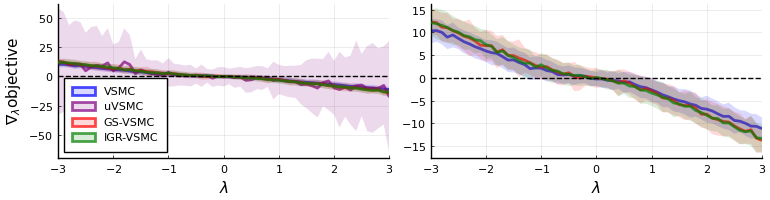
\includegraphics[width=\textwidth]{figures/grad_est_var.png}
\caption{\textbf{(Left)} Mean and standard deviation over 100 gradient estimates for varying values of $\lambda$ for a single scalar linear Gaussian \ssm problem. The number of particles is $N=2$. The optimal value of $\lambda$ is the point at which the mean gradient is 0. \textbf{(Right)} The same figure but without \uvsmc for better visibility.}
\label{fig:grad_est_var}
\end{figure}

We consider the scalar linear Gaussian \ssm problem with $A=0.5$, $Q=1$, $C=1$, $R=1$, and $T=2$. Following \textcite{Naesseth:2018}, we use the proposal $q_\lambda(x_t|x_{t-1}) = \mathcal{N}(\lambda+0.5x_{t-1}, 1)$ with $\lambda\in\mathbb{R}$ and $x_0=0$. We use $N=2$ particles to approximate the posterior.
\\

\textbf{Variance of gradient estimator.} We first investigate whether our proposed extension reduces the variance of the unbiased \elbo gradient estimator. Figure~\ref{fig:grad_est_var} shows the mean and the standard deviation over 100 gradient estimates as $\lambda$ varies for a single generated dataset. The four gradient estimators are \vsmc ($\grep$), \uvsmc ($\grep+\gscore$), \gsvsmc (\vsmc with \gumbelsoftmax), and \igrvsmc (\vsmc with \igr). The observed behaviour of \vsmc and \uvsmc are similar to what was observed with $\grep$ and $\gscore$ in \parencite{Naesseth:2018}, though we note that the standard deviations of our estimators appear to be larger than what they observed (for $N=2$). We were unable to find the source of this difference in spread, but we suspect it to be a numerical stability issue coming from automatic differentiation. The figure clearly shows that \gsvsmc and \igrvsmc reduce the variance of the unbiased gradient estimator (\uvsmc), and that the behaviour of \gsvsmc and \igrvsmc are very similar to that of the biased gradient estimator (\vsmc).
\\

\begin{figure}[t]
\centering
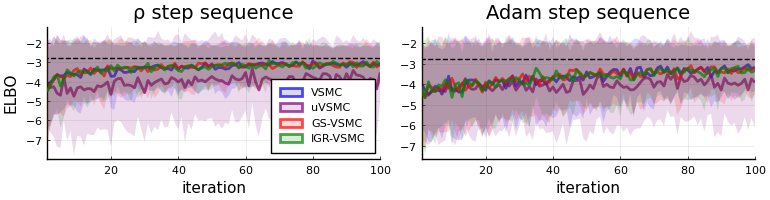
\includegraphics[width=\textwidth]{figures/slgss_elbo.png}
\caption{Mean and standard deviation of the estimated \elbo for a scalar linear Gaussian \ssm problem across 100 runs with different step sequences. The black line is the log marginal likelihood $\log p(y_{1:T})$.}
\label{fig:slgss_elbo}
\end{figure}

\textbf{Tightness of \elbo estimate.} We next evaluate how tight of a lower bound our proposed extension is able to estimate. Figure~\ref{fig:slgss_elbo} shows the mean and standard deviation of the estimated \elbo across 100 runs. Following \textcite{Naesseth:2018}, we try both the Adam step sequence and the adaptive $\rho$ step sequence \parencite{Kucukelbir:2017} given by
\begin{align*}
\rho^k &= \eta k^{-1/2+\delta}(1+\sqrt{s^k})^{-1} \\
s^k &= t\left(\hat{\nabla}\tilde{\mathcal{L}}(\lambda^k)\right)^2+(1-t)s^{k-1}
\end{align*}
where $k$ is the iteration number, $\delta=10^{-16}$, $t=0.1$, and $\eta=0.1$. We find that all four methods are able to closely estimate the \elbo after a reasonable number of iterations, although \vsmc with the unbiased gradient takes notably longer to converge. There is no obvious difference between \vsmc, \gsvsmc, and \igrvsmc. We also note that using the $\rho$ step sequence appears to converge faster than Adam and so we use the $\rho$ steps in our following experiments unless otherwise specified.
\\

\textbf{Role of $\tau$.} We also investigate the role of the temperature $\tau$ specifically in \gsvsmc. We use the same scalar linear Gaussian \ssm setting but with $T=4$. Figure~\ref{fig:tau_plots} shows the mean and standard deviation of the \elbo gradient estimate as well as the mean and standard deviation of the \elbo estimate for \gsvsmc with three levels of $\tau$. We observe that the standard deviation of the gradient estimator can become unstable for very small $\tau$ (e.g., $\tau=0.001$). Higher mixing rates appear to have a greater impact on the estimation of the \elbo when the number of particles is large (e.g., $N=50$), but the impact is arguably marginal considering the relative error. Our results suggest that using a $\tau$ ``small enough'' (e.g., $\tau=0.1$) is likely sufficient for reasonable estimation.

\begin{figure}[t]
\centering
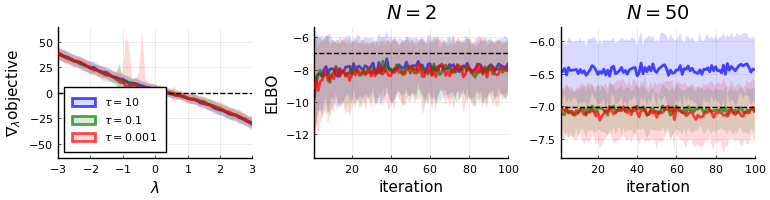
\includegraphics[width=\textwidth]{figures/tau_plots.png}
\caption{\textbf{(Left)} Mean and standard deviation over 100 gradient estimates of \gsvsmc with different values of $\tau$ for a scalar linear Gaussian \ssm problem. \textbf{(Center, Right)} Mean and standard deviation over 100 \elbo estimates of \gsvsmc with different values of $\tau$ and using $N$ particles.}
\label{fig:tau_plots}
\end{figure}

\subsection{Linear Gaussian \ssm}

We evaluate our proposed extension on higher dimensional linear Gaussian \ssm problems. We use the model parameters $(A)_{i,j}=\alpha^{|i-j|+1}$ where $\alpha=0.42$, $Q=I$, $R=I$, $C\sim\mathcal{N}(0,I)$, and $T=10$. We try two settings of $d_x=\dim(x_t)$ and $d_y=\dim(y_t)$. We use the proposal
\[
q_\lambda(x_t|x_{t-1}) = \mathcal{N}\left(\mu_t+\mathrm{diag}(\beta_t)Ax_{t-1},\mathrm{diag}(\sigma_t^2)\right)
\]
and approximate the target with $N=4$ particles.
\\

Figure~\ref{fig:lgss_elbo} shows the mean and standard deviation of the \elbo estimate for \vsmc, \uvsmc and \gsvsmc over 100 runs. Note that we found the optimization step of \igrvsmc to be prohibitively expensive in this context and so we did not consider it. We also found that \uvsmc converged at a much slower in this context (if at all), though we note that we did not fine tune the step sizes beyond trying the Adam and $\rho$ step sequences. The performance of \gsvsmc seems comparable to \vsmc in the first setting but a more notable difference is present in the second setting. We suspect that the target may be more multimodal in higher dimensions and so taking mixtures may more likely result in proposals in regions of low density. It may be necessary to lower $\tau$ to compensate in this case. We note this as a possible limitation of our proposed extension.

\begin{figure}[t]
\centering
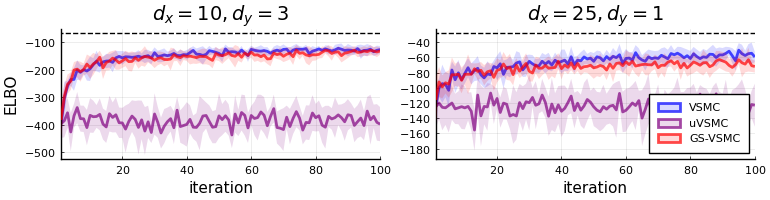
\includegraphics[width=\textwidth]{figures/lgss_elbo.png}
\caption{Mean and standard deviation of the estimated surrogate \elbo across 100 runs for two linear Gaussian \ssm problems. The black line is the log marginal likelihood $\log p(y_{1:T})$. Here, \uvsmc uses the Adam step sequence.}
\label{fig:lgss_elbo}
\end{figure}

\subsection{Capital Asset Pricing Model}

We lastly compare our proposed extension to \vsmc for modeling the \textsc{RPMF} data in the Capital Asset Pricing Model (\capm) dataset \parencite{Verbeek:2004}. The dataset contains the approximate excess return (expressed in percentage per month) on the market portfolio for the period January 1960 to December 2002 (516 months). A \ssm is reasonable for modeling the data due to abnormal patterns in the returns that cannot be explained by the single-factor CAPM. To model the data, we use the same scalar linear Gaussian \ssm and proposal explored in our previous experiments but with $T=516$ and $N=8$. Note that in this setting, we learn the model parameters along with the variational parameter $\lambda$ in what \textcite{Naesseth:2018} describe as \textit{variational expectation-maximization}. Both the surrogate \elbo and our estimate of the \elbo is updated in each iteration of this procedure.
\\

Figure~\ref{fig:capm_plots} shows the estimated \elbo over training, as well as the \capm dataset along with three samples generated by \vsmc, \gsvsmc, and \igrvsmc. Each sample was generated by first sampling a sequence $x_{1:T}$ from \smc with the learned proposal, and then sampling $y_t\sim \mathcal{N}(Cx_t,R)$ for $t=1,...,T$ using the learned model parameters $C$ and $R$. We observe that even with the relatively simple model, all three methods are able to capture the general patterns in the data and produce samples that arguably resemble the original data. Qualitatively, we do not observe obvious differences between \vsmc and our approximating versions. Quantitatively, we compare the trained methods using the normalized effective sample size defined as
\[
\text{normalized ESS} = \frac{1}{N\sum_{i=1}^N(w_T^i)^2}
\]
which can be computed using the weights obtained as a byproduct of running \smc. We find that the mean and standard deviation of the normalized \textsc{ESS} over 100 sample \elbo estimates is $\mathbf{0.340\pm0.115}$ for \vsmc, $\mathbf{0.353\pm 0.116}$ for \gsvsmc, and $\mathbf{0.274\pm0.093}$ for \igrvsmc.

\begin{figure}[t]
\centering
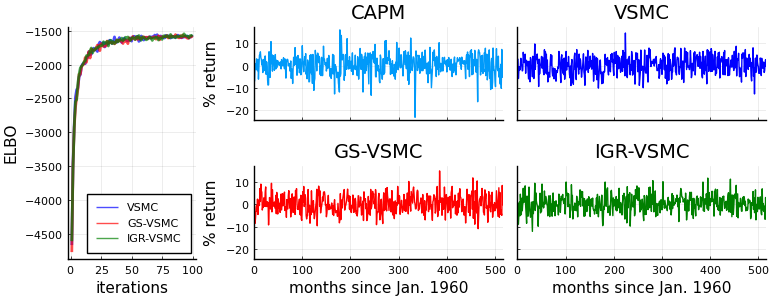
\includegraphics[width=\textwidth]{figures/capm_plots.png}
\caption{\textbf{(Left)} The estimated \elbo over training for the \capm dataset. \textbf{(Right)} The \capm dataset of returns on the market portfolio and one sample generated from each of \vsmc, \gsvsmc, and \igrvsmc.}
\label{fig:capm_plots}
\end{figure}


\section{Discussion}\label{sec:discussion}

We have highlighted the main contributions and limitations of the paper by \textcite{Naesseth:2018} and reviewed their proposed \vsmc method. We proposed using a continuous, reparameterizable approximation to the \categorical resampling procedure in \vsmc to help reduce the variance of the unbiased gradient estimator. Our experimental results suggest that the \gumbelsoftmax approximation leads to a \gsvsmc performance that is comparable to that of standard \vsmc with the biased gradient estimator. The benefit of \gsvsmc over \vsmc is that the model being optimized and the model used at run time are identical, and so the possibility of a solution optimization gap is less of a concern (up to stochastic optimization confidence). Although \gsvsmc is not exact \smc and the \elbo objective is only approximate, we find that the difference is negligible as long as $\tau$ is ``small enough''. Our investigation of $\tau$ suggests that a value on the magnitude of $0.1$ is sufficient for achieving reasonable estimation in a simple linear Gaussian \ssm problem. We suspect that this value may need to be lower for complex problems in higher dimensions, which may be a limitation of our proposed extension.
\\

We also explored using the \igr approximation in \vsmc but found the necessary optimization problem for fitting the \igr parameters to be a computational bottleneck. We ran \igrvsmc in our experiments by sacrificing optimization accuracy and its results were subpar or comparable to the other methods at best. However, we believe the \igr approximation has potential due to its promise of being more flexible than the \gumbelsoftmax. We expect that significant gains can be obtained if a closed form for the inner optimization is available through careful choices of the reparameterized distribution and the invertible transformation.


\newpage

\printbibliography

\end{document}